\documentclass[12pt,a4paper]{article}
%\documentclass[12pt,a4paper, titlepage]{article}

\usepackage{graphicx}

\usepackage{gensymb}

\usepackage{ifthen}

\usepackage{listings}

% For hypertext links in pdf and dvi files
\usepackage{hyperref}

\usepackage{asymptote}

\title{INCL cascade}

\author{Pekka Kaitaniemi} 
\date{\today}

\graphicspath{{.}{images/}}

\begin{document}
\maketitle

\section{Introduction}

This is the C++ version of the INCL4 cascade model version 4.2. The
original FORTRAN version of this model is developed at CEA \cite{cea}
and Li\`ege \cite{liegeuniversity} university. We have been working
together with the original developers and our contact person is Alain
Boudard at CEA/Saclay. The code translation project has been done at
Helsinki Institute of Physics.

\section{INCL cascade}

\subsection{Features}

The INCL4 cascade can be used to simulate the collisions between
bullet particles and nuclei. The supported bullet particles and the
interface classes supporting them are presented in table
\ref{tbl:bullets}.

\begin{table}
\caption{Bullet particles supported by the INCL4 cascade and the
  related interface classes.}
\label{tbl:bullets}
\begin{center}
\begin{tabular}{|c|c|c|}
\hline
Geant4 interface & Type & Particle \\
\hline
G4InclCascadeInterface & Nucleons & Proton \\
 &                                & Neutron \\
 &                       Pions    & $\pi^+$, $\pi^0$, $\pi^-$ \\
\hline
G4InclLightIonInterface & Light ions & Deuteron \\
 &                                    & Triton \\
 &                                    & He3 \\
 &                                     & Alpha \\
\hline
\end{tabular}
\end{center}
\end{table}

The momenta and positions of the nucleons inside the nuclei are
determined at the beginning of the simulation run by modeling the
nucleus as a free fermi gas in a static potential well. The cascade is
modeled by tracking the nucleons and their collisions. The collisions
are assumed to be well separated in space and time.

The possible reactions inside the nucleus are 
\begin{itemize}
\item $NN \rightarrow N \Delta$ and $N \Delta \rightarrow NN$ 
\item $\Delta \rightarrow \pi N$ and $\pi N \rightarrow \Delta$
\end{itemize}

\begin{figure}[ht]
\begin{center}
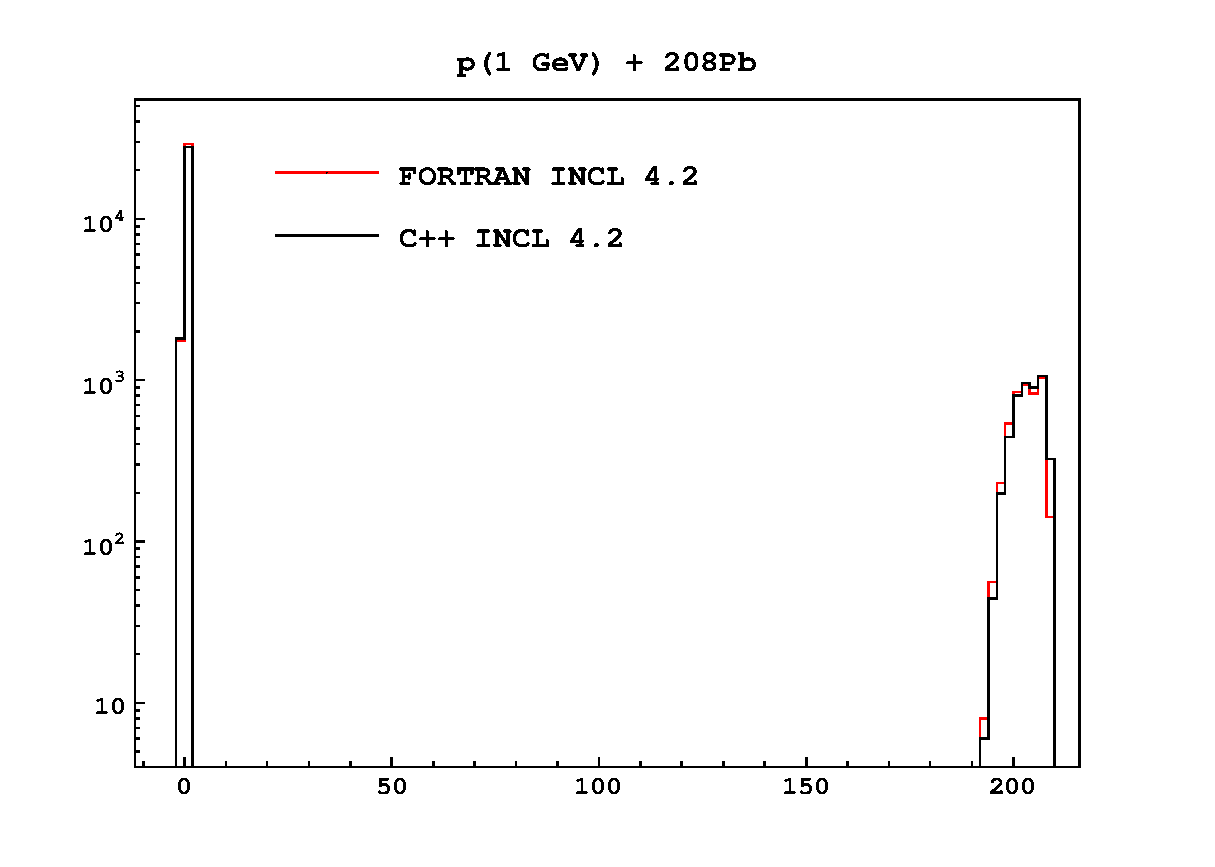
\includegraphics[scale=0.6]{Pb208Proton1GeV.eps}
\end{center}
\caption{Colliding 1 GeV proton to Pb208 target. Here is presented the
mass number of the outcoming particles.}
\end{figure}

\subsection{Model limits}

The INCL4 model has certain limitations with respect to the bullet
particle energy and target nucleus type. The supported energy range
for bullets is: 200 MeV - 3 GeV. Acceptable target nuclei range from
Carbon to Uranium.

\section{ABLA 3.0 data G4ABLADATA}

INCL and ABLA for Geant4 9.1 need data files for mainly shell
corrections and for INCL mass of the remnant nucleus. To enable this
dataset environment variable {\tt G4ABLADATA} needs to be set and the
data downloaded from Geant4 web page. For Geant4 9.1 release use ABLA
version 3.0.

\begin{thebibliography}{99}
\bibitem{incl1} J. Cugnon et al \emph{Nuc. Phys. A352} (1981) 505
\bibitem{incl2} J. Cugnon et al \emph{Nuc. Phys. A462} (1987) 751
\bibitem{incl3} J. Cugnon et al \emph{Nuc. Phys. A500} (1989) 701
\bibitem{incl4} A. Boudard et al \emph{Phys. Rev. C66} (2002) 044615
\bibitem{liegeuniversity} Li\`ege University
\href{http://www.ulg.ac.be/foreign/}{{\tt http://www.ulg.ac.be/foreign/}}
\bibitem{cea} CEA website
  \href{http://www.cea.fr/gb/index.asp}{{\tt http://www.cea.fr/gb/index.asp}}
\end{thebibliography}

\end{document}